% Lecture 1
% Daniel Ellison 2019
% LaTeX

%%%%%%%%%%%%%%%%%%%%%%%%%%%%%%%%%%%%%%
\part*{Lecture 1: \\Arithmetic, Variables, Strings, Booleans, If/Else Statements}


\section*{What is computer science about?}

In this course you’re going to learn how to write useful programs and think like a computer scientist.

Since you’ll be learning to control computers, let’s get oriented with a brief look at a typical computer system. 

%% \begin{center}
%% \includegraphics[width=10cm]{picture of computer setup}
%% \end{center}

At the center of our picture we have the central processing unit, or CPU, which is like the brain. The CPU can store and process its own data --- or exchange data with connected devices. If you browse the internet using wifi, for example, the CPU is sending data to your wireless port to request webpages, receiving website data from your wireless port, processing that data, and sending images to your monitor to for display. 

At the hardware level, all this data consists of 0s and 1s (\emph{bits}), which are stored in chunks called words (32 and 64-bit words are typical of modern devices). The CPU has many addresses where words may be stored and the CPU hardware supports a \emph{machine language} of commands to manipulate words. For example, a machine language command might be used 
to move a word at one address to different address; or to add one word to another. It turns out that machine language instructions are themselves stored as words with addresses, and machine languages typically support commands like ``execute the command at address 57 if the word at address 2 is all 0s". 

%% \begin{center}
%% \includegraphics[width=10cm]{picture of addresses and words}
%% \end{center}

If you’re thinking it would be a nightmare to get a computer to do anything useful with machine language, you’re not alone. It would be much more convenient for a programmer to be able to write a program in a \emph{higher-level} language, one closer to human language. In the 1950’s, computer scientists began to make this possible, developing programs, which, given a program written in a higher-level language, would carry out the program’s intent by systematically translating it to machine language --- which is all the CPU really understands. 

In this course you’ll learn computer science with Python, a high level language which was first released by Dutch Programmer Guido van Rossum in 1990. Python is now on version 3.7.3 and is widely used both in university courses and industry. Once you learn to express yourself in one programming language it’s much easier to pick up another, so the Python you learn will be useful to you in any future programming—from using C to control embedded systems to doing engineering programming in MatLab.


\section*{Administrative Details}

I’ll be teaching the course for the first 2 weeks and David Thorpe, a professional software engineer, will teach for the second 2 weeks (but I’ll stick around as your TA). 

Here’s the class structure for the first 2 weeks. We’ll begin with a brief introduction to the days topics, and the majority of the class will be an in-class mini-project --- a short programming project to give you practice writing useful programs. 

Beginning next class (Wednesday), each class will also begin with a short (5-10 min) quiz to check that you’re up to speed. If you understand the mini-projects and lectures you should be good to go. If not, come find me and ask for help. I’ll do my best help you figure things out.


\section*{But let’s get to learning Python!}

We’ll be using the IDLE development environment. When you open the IDLE application you find yourself in a window like this:

\begin{center}
	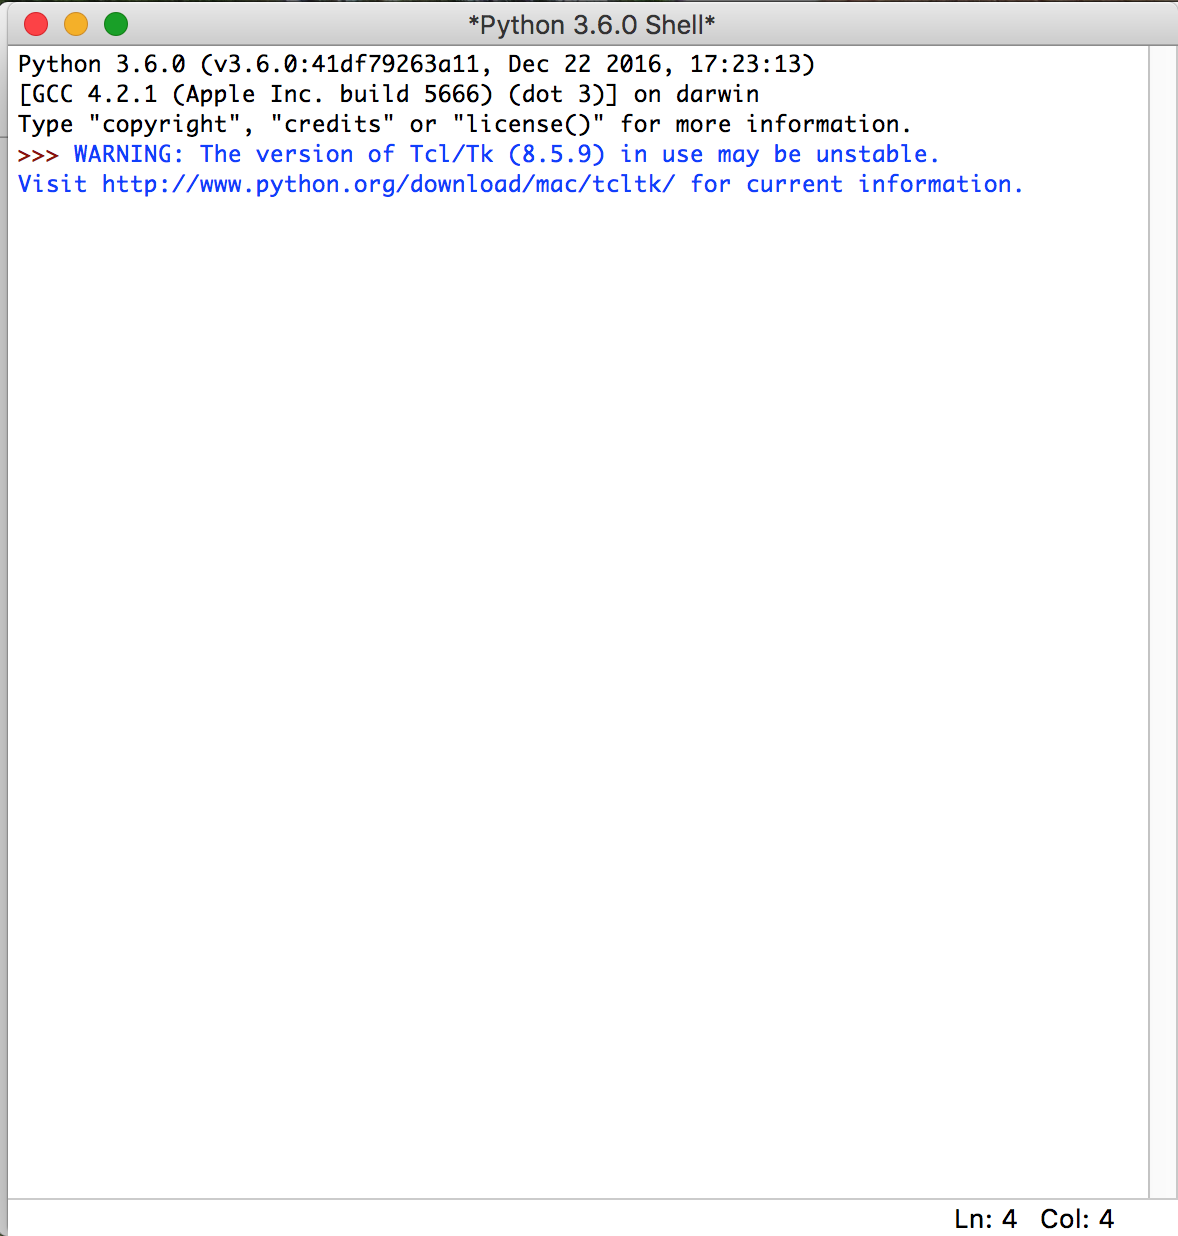
\includegraphics[width=10cm]{blank_idle}
\end{center}

This is a python shell --- kind of like the Terminal on Macs if you’ve used that. You type in an instruction and press enter to run it. If you’ve phrased your command properly, the shell will print out the result --- otherwise the shell will give you an error message. The shell is kind of like a playground where you can run programs one piece at a time to make sure your commands are doing what you think. We’ll get to writing and executing full python files in a bit. In the meantime let’s take the opportunity to learn a bit of the Python language and practice using the shell.


\section*{Arithmetic}

We’ll start with some arithmetic. Perhaps unsurprisingly, Python can do anything your standard calculator can do. Typing in \texttt{4+5}, for example, and pressing enter will cause the shell to print \texttt{9}, the result.

\begin{lstlisting}[numbers=none]
>>> 4 + 5 
9
\end{lstlisting}

You can use all the standard math operations: \texttt{+}, \texttt{-}, \texttt{*} (multiplication), \texttt{/} (division), and \texttt{**} (exponentiation).

\begin{lstlisting}[numbers=none]
>>> 4 + 5 / 4 * 7 - 9
3.75
\end{lstlisting}

Python uses the standard order of operations, but if order of operations is a concern, you can use parentheses to be explicit.

\begin{lstlisting}[numbers=none]
>>> 4 + 5 / (4 * 7) - 9
-4.821428571428571
\end{lstlisting}

Python also supports some arithmetic functions you might not find on a calculator, such as the modulo operator (python uses the symbol \texttt{\%}). \texttt{x \% y} gives the remainder when x is divided by y. 

\begin{lstlisting}[numbers=none]
>>> 5 % 3
2
\end{lstlisting}

Incidentally, some operations on your scientific calculator (for example cos, sin, tan) won’t run if you type them in. 

\begin{lstlisting}[numbers=none]
>>> cos(90)
Traceback (most recent call last):
  File "<pyshell#5>", line 1, in <module>
    cos(90)
NameError: name 'cos' is not defined
\end{lstlisting}

This is because the function ``cos" is not part of the Python language—so I lied by saying that python can do everything your calculator can. But it’s only a little lie. People have written a Python library, the math library, which you can use to make the cosine function available.

\begin{lstlisting}[numbers=none]
>>> from math import cos
>>> cos(90)
-0.4480736161291701   
\end{lstlisting}   

Looks like the math library uses radians… The math library is always available with Python, so it’s almost as good as having cosine be part of the Python language itself. We’ll talk more about libraries and how they work (and how you can write your own) in a lecture 3.


\section*{Variables and Assignment, Types}

Most of the time, after doing some arithmetic, you’ll want the computer to keep track of the computed value so you can work with it further. To do this you can \emph{assign} the value to a \emph{variable}. (recall \texttt{**} is Python’s exponentiation operator)

\begin{lstlisting}[numbers=none]
>>> really_big_number = 2 ** 100
\end{lstlisting}

When you assign a variable, the shell won’t print out the value of the variable, but, if you want to see it, you can enter the variable name into the shell. 

\begin{lstlisting}[numbers=none]
>>> really_big_number
1267650600228229401496703205376
\end{lstlisting}

You can then use the variable in further commands and the shell will treat it just as if you put in the variable’s value (126…76) instead of its name.

\begin{lstlisting}[numbers=none]
>>> really_big_number * 10 + 2
12676506002282294014967032053762
\end{lstlisting}

We can even define one variable in terms of another.

\begin{lstlisting}[numbers=none]
>>> tshirts_at_home = 14
>>> tshirts_thrown_out = 2
>>> tshirts_remaining = tshirts_at_home - tshirts_thrown_out
>>> tshirts_remaining
12
\end{lstlisting}

You can name a variable almost anything you want, as long as it follows the following two rules:
\begin{enumerate}
\item The variable name cannot be a reserved word in the Python language (such as \texttt{for}, \texttt{while}, \texttt{if}, \texttt{True}, and a few others). Luckily, IDLE turns these words different colors (try it!) so it’s not hard to avoid this mistake.

\item The variable name begins in a letter or underscore (\texttt{\_}) and continues with some combination of letters, numbers, and underscores. (so I couldn’t use the name \texttt{t-shirts\_thrown\_out}, for example, since it contains a hyphen.
\end{enumerate}

In this course, we’ll use the typical convention of naming variables as single lower case words, or a number of lower-case words separated by underscores.

So what is \texttt{tshirts\_remaining}? It’s a variable. But what kind of variable, what sort of value does it have? Let’s ask Python, using the \texttt{type} function.

\begin{lstlisting}[numbers=none]
>>> type(tshirts_remaining)
<class 'int'>
\end{lstlisting}

We’ll get to Python’s class system later in the course, but the shell is telling us that the value of the variable \texttt{tshirts\_remaining} is of type \texttt{\textquotesingle int\textquotesingle} --- an integer. This is because 12 is an integer (a fancy word for whole number). Python has a number of different types. We’ve already seen numbers that aren’t integers, let’s find out their type...

\begin{lstlisting}[numbers=none]
>>> non_whole_number = .34758
>>> type(non_whole_number)
<class 'float'>
\end{lstlisting}

Numbers which aren’t integers (whole numbers) are of type \texttt{\textquotesingle float\textquotesingle}. This is short for `floating point number', because the number has a decimal point.

Python’s type system distinguishes the different types of data you can work with when programming. So far we have whole numbers (\texttt{\textquotesingle int\textquotesingle}) and decimals (\texttt{\textquotesingle float\textquotesingle}). There are many others types in Python (you’ll even learn to build your own types in lecture 4). Today we’ll learn two more you can use in your programs --- \texttt{\textquotesingle str\textquotesingle} (strings of text) and \texttt{\textquotesingle bool\textquotesingle} (can either be \texttt{True} or \texttt{False}).



\section*{Strings, Print, and Input}

Strings are chunks of text, like \texttt{\textquotesingle Eat healthy\textquotesingle}, or \texttt{\textquotesingle clean your room!\textquotesingle}, or\\ \texttt{\textquotesingle…;a94302\textquotesingle}. More formally, a string is a sequence of characters. \texttt{\textquotesingle Eat healthy\textquotesingle}, for example, begins with the character \texttt{\textquotesingle E\textquotesingle}, and continues with \texttt{\textquotesingle a\textquotesingle}, \texttt{\textquotesingle t\textquotesingle}, \texttt{\textquotesingle\textvisiblespace\textquotesingle}, \texttt{\textquotesingle h\textquotesingle}, and so on. 

You can assign a variable to have a string value just like we assigned a variable to have an int or float value:

\begin{lstlisting}[numbers=none]
>>> current_location = 'Barbados'
\end{lstlisting}

If we wanted to check the value of \texttt{current\_location}, we can just type it into the shell and press enter, like with numbers.

\begin{lstlisting}[numbers=none]
>>> current_location
'Barbados'
\end{lstlisting}

This is a fine way to see the value of the \texttt{current\_location} variable, but the problem is it only works in the shell. Let’s learn a way to display a string variable that always works --- the \texttt{\textbf{ print}()} function.

\begin{lstlisting}[numbers=none]
>>> print(current_location)
Barbados
\end{lstlisting}

Pretty straightforward. In fact, the print function can be used to display the value of an integer variable.

\begin{lstlisting}[numbers=none]
>>> print(tshirts_remaining)
12
\end{lstlisting}

I’ve made it seem like you can only print variables, not strings or numbers themselves; but if it works with the variable, it will work with the value. That’s a pretty universal fact in Python.

\begin{lstlisting}[numbers=none]
>>> print('encyclopedia')
encyclopedia
\end{lstlisting}

Really, the print function only knows how to print strings (objects of type \texttt{\textquotesingle str\textquotesingle}). When asked to print an \texttt{\textquotesingle int\textquotesingle} like 12, it performs a \emph{type conversion} behind the scenes to turn the integer into a string. How does it do that? Well, it makes a string out of the \emph{digits} of the number, concatenating \texttt{\textquotesingle1\textquotesingle} and \texttt{\textquotesingle2\textquotesingle} to make \texttt{\textquotesingle12\textquotesingle}. \texttt{\textquotesingle12\textquotesingle} is a string, and the print function knows how to display strings. This might seem like I’m making a mountain out of a molehill, but type conversion is a very useful concept --- take the time to understand this paragraph. There really is a difference between the integer \texttt{12} and the string \texttt{\textquotesingle12\textquotesingle}!

%% The conversion of numbers (\ttexttt{\textquotesingle float\textquotesingle} and \texttt{\textquotesingle int\textquotesingle}) to strings arises frequently in programming, and it’s not just the print function which can do it. You can use the \texttt{\textbf{ str}()} function MAYBE GET RID OF

Python also supports a number of operations on strings. One is concatenation, which forms a new string by putting one directly after another. Python uses the \texttt{+} symbol to concatenate strings. The syntax is just like adding numbers:

\begin{lstlisting}[numbers=none]
>>> mystery_animal = 'mountain' + 'lion'
>>> print(mystery_animal)
mountainlion
\end{lstlisting}

Why didn’t python add a space between the two words? Because we didn’t tell it to add one. A space is a character like any other in a Python string and you must add it explicitly when concatenating strings.

\begin{lstlisting}[numbers=none, showstringspaces=true]
>>> mystery_animal_fixed = 'mountain' + ' ' + 'lion'
>>> print(mystery_animal_fixed)
mountain lion
\end{lstlisting}

Python also supports string ‘splicing’, which means picking out characters in a string. For example, if we wanted to print the \texttt{\textquotesingle o\textquotesingle} in the string \texttt{\textquotesingle Barbados\textquotesingle}, we could do the following.

\begin{lstlisting}[numbers=none]
>>> country = 'Barbados'
>>> print(country[6])
o
\end{lstlisting}

As the above example shows, the syntax for selecting a single character from a string is to follow the string variable with brackets containing the position of the chosen character. This position is called the index of the character. But hold on a second! \texttt{\textquotesingle o\textquotesingle} isn’t the 6th letter of Barbados. Is there a typo in the notes? The reason is that Python begins counting at 0, not 1. So the character at index \texttt{0} is \texttt{\textquotesingle B\textquotesingle}, the character at index \texttt{1} is \texttt{\textquotesingle a\textquotesingle}, the character at index \texttt{2} is \texttt{\textquotesingle r\textquotesingle}, and so on. 

One final note on strings. When writing programs, you might want to obtain information from a user --- such as their name --- and store it as a variable. To do this you can use the input function:

\begin{lstlisting}[numbers=none]
>>> name = input('Please enter your name: ')
Please enter your name: Matt             <--- I typed in my name here
>>> print('Welcome ' + name)
Welcome Matt
\end{lstlisting}

Give it a try. It will prompt you for your name, which you type in and press enter. After that, the entered text will be assigned to the variable \texttt{name}, which you can use later in your program.



\section*{Interlude: Break Out of the Shell!}

It probably feels silly typing your programs in one line at a time. The shell is useful for testing that things are working the way you want—but if you’re writing a real Python program, you’ll write it as its own .py file (or even as multiple .py files, but we’re not there yet).

First, open up a new python file.

\begin{center}
	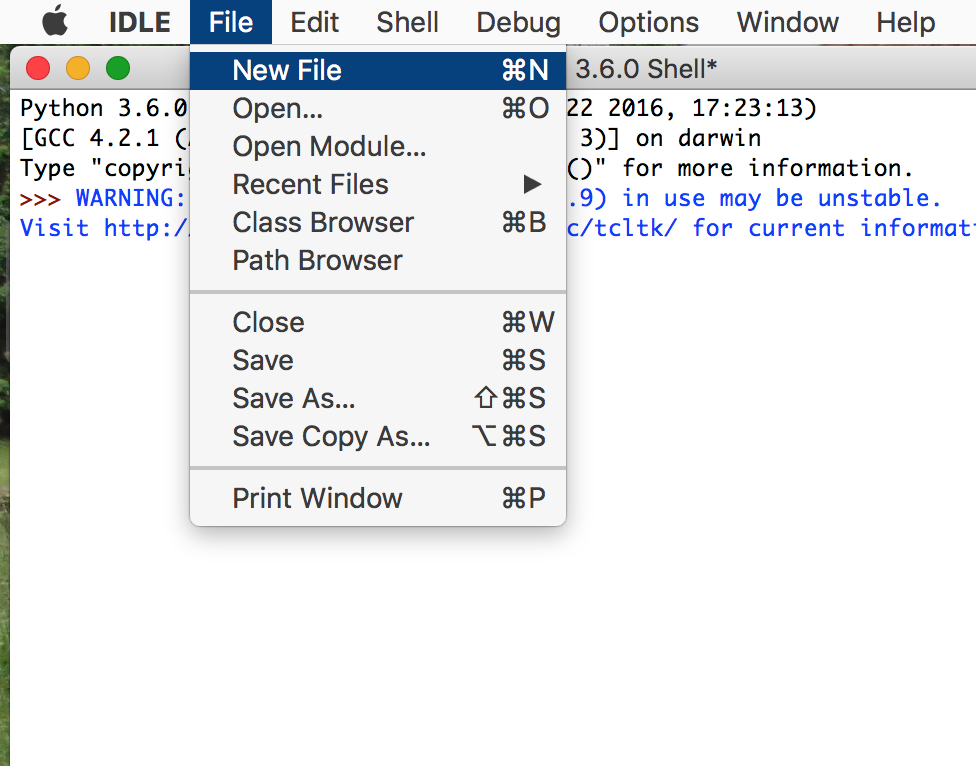
\includegraphics[width=10cm]{new_file}
\end{center}

This will pull up a window where you can write your program. As an example, feel free to type in the following

\begin{lstlisting}
name = input('Please Enter Your Name: ')
print(name + '. Hello again!')
\end{lstlisting}

To run your program, select Run ---$>$ Run Module

\begin{center}
	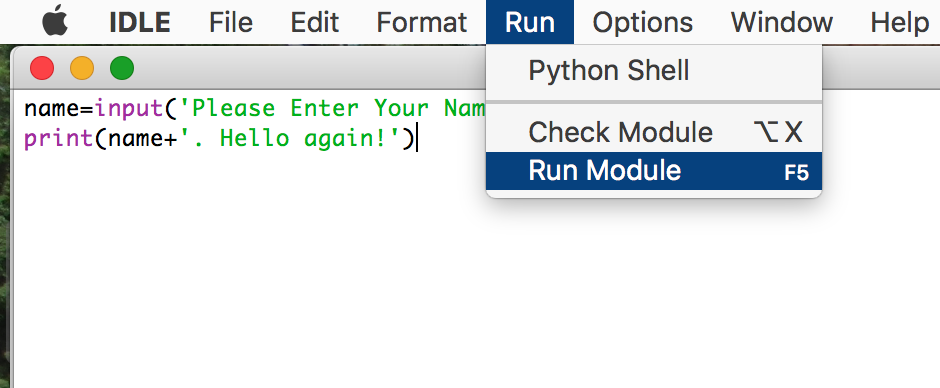
\includegraphics[width=10cm]{run_module}
\end{center}

Idle will then prompt you to save your file as a .py file, and once you do so, it will run it in the shell. If Python can’t understand your program (for example, if you mistype a command like print), your program won’t run and IDLE will try to explain what went wrong.

This will be our program-writing process for the rest of the course, but don’t feel shy about using the shell to test or double-check small ideas! For example, if you’re wondering whether the character at index \texttt{2} of \texttt{\textquotesingle music\textquotesingle} is \texttt{\textquotesingle u\textquotesingle} or \texttt{\textquotesingle s\textquotesingle}, it’s easiest to just plug the following command into the shell. 

\begin{lstlisting}[numbers=none]
>>> 'music'[2]
's'
\end{lstlisting}


\section*{Booleans and if/else}

You’ve learned a lot already, and we’ll finish up today’s lecture with one more piece of the Python language --- one that allows your programs to make decisions. For example, you might write a program to ask for the user’s password, and, \emph{if it’s correct}, admit the user. \emph{Otherwise}, the program can print out \texttt{\textquotesingle incorrect password\textquotesingle}.

The standard way to make these True/False decisions is with an \texttt{if}/\texttt{else} clause (run this as a .py file):

\begin{lstlisting}
secret_password = 'bluetoad'
entered_password = input('Please Enter The Password to Continue: ')
if entered_password == secret_password:
	print('Correct. Welcome!')
else:
	print('Incorrect Password.')
\end{lstlisting}

This piece of code begins by asking the user to enter a password with the input function. The entered password is stored as the variable \texttt{user\_password}. Then, the program compares the entered password to the real password.

This is done by the comparison operator, \texttt{==}, which tests whether the two strings are same.

If the comparison operator gives \texttt{True} (meaning the strings are the same), the program moves on to the part after \texttt{if}. Otherwise, the program moves on to the part after \texttt{else}.

The general form of an \texttt{if}/\texttt{else} clause is as follows:

\begin{verbatim}
if [an expression --- either true or false]:
    [commands to follow if the expression is true]
else:
    [commands to follow if the expression is false].
\end{verbatim}

Let’s dig deeper into the `an expression—either true or false' bit. The use of \texttt{==} to compare two strings provides one example. Another example might be the following:

\begin{lstlisting}
my_number = 10
if my_number % 2 == 0:
	print('your number is even')
else:
	print('your number is odd')
\end{lstlisting}

The expression \texttt{my\_number \% 2 == 0}, divides \texttt{my\_number} by \texttt{2} and takes the remainder (the \texttt{my\_number \% 2} part does this), then compares the result (either \texttt{0} or \texttt{1}) to \texttt{0}. If they are equal, this means \texttt{my\_number} is even, and the program says so. Otherwise, the program prints that the number is odd.  

So the expression \texttt{my\_number \% 2 == 0} is either \texttt{True} or \texttt{False}, depending on the value of \texttt{my\_number}. Such expressions which may be \texttt{True} or \texttt{False} are known as \emph{booleans} (of type \texttt{\textquotesingle bool\textquotesingle}). Python will tell you this, too, if you ask.

\begin{lstlisting}[numbers=none]
>>> my_number = 10
>>> type(my_number % 2 == 0)
<class 'bool'>
\end{lstlisting}

Once the computer evaluates a boolean, it will give either \texttt{True} or \texttt{False}, and you can assign the value to a variable. If you already know which it should be, you can simply define a variable as \texttt{True} or \texttt{False} directly (python insists on uppercasing \texttt{True} and \texttt{False} in this case).

\begin{lstlisting}[numbers=none]
>>> its_raining = False
>>> i_have_no_umbrella = True
\end{lstlisting}

Such true/false expressions may also be built together using \texttt{or} and \texttt{and} in much the same way as english:

\begin{lstlisting}[numbers=none]
>>> my_clothes_are_soaked = its_raining and i_have_no_umbrella
>>> print(my_clothes_are_soaked)
False
>>>
>>> i_have_a_dog = False
>>> i_have_a_parrot = True
>>> i_have_a_pet = i_have_a_dog  or i_have_a_parrot
>>> print(i_have_a_pet)
True
\end{lstlisting}

To be more explicit, the expression \texttt{X and Y} is \texttt{True} only if both \texttt{X} and \texttt{Y} are \texttt{True} --- and \texttt{False} otherwise. The boolean \texttt{X or Y} is \texttt{True} unless both \texttt{X} and \texttt{Y} are \texttt{False}—that is if \texttt{X} or \texttt{Y} is \texttt{True}, or they’re both \texttt{True}.

Booleans can also be modified with the \texttt{not} keyword. If you put \texttt{not} before a boolean \texttt{X} it gives the reverse. So \texttt{not X} is \texttt{True} if \texttt{X} is \texttt{False}, and \texttt{False} if \texttt{X} is \texttt{True}.

\begin{lstlisting}[numbers=none]
>>> sent_delivery = True
>>> didnt_send_delivery = not sent_delivery
>>> print(didnt_send_delivery)
False
\end{lstlisting}

These compound booleans, using \texttt{and}, \texttt{or}, \texttt{not} can be put into \texttt{if}/\texttt{else} expressions in the same way:

\begin{lstlisting}
on_beach = True
have_work = False
if on_beach and (not have_work):
	print('on vacation!')
else:
	print('not on vacation...')
\end{lstlisting}

Alright, if you’ve followed all this give yourself a pat on the back! You’re well on the way to writing interesting programs. The best way to develop skill as a programmer is to write programs---so let’s go onto the first mini-project. 

Since we covered a lot of introductory material today, the mini project is short. In later lectures, we’ll have less introductory material to cover and you’ll get to work on more interesting programs.
